\documentclass[../main.tex]{subfiles} 
\begin{document}
		O trabalho prevê o projeto e implementação, através de código de descrição de hardware (VHDL),
		de um microprocessador com arquitetura multiciclo e um número reduzido de instruções, de acordo com a 
		tabela da figura~\ref{fig:tabela_instrucoes}
		
		\begin{figure}[h]
			\centering
			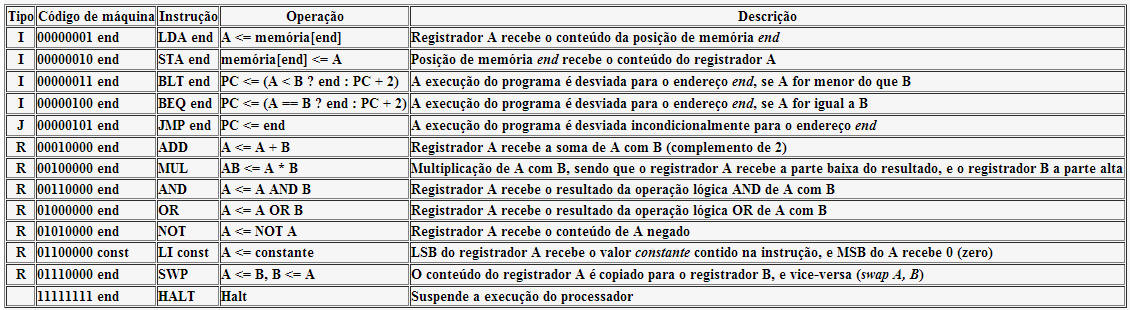
\includegraphics[width=\textwidth]{img/tabela_instrucoes}
			\caption{Tabela com a especificação das instruções que devem rodar no microprocessador}
			\label{fig:tabela_instrucoes}
		\end{figure}
		
		O processador projetado deve executar um programa exemplo descrito em linguagem Assembly.
		
		O processador implementado foi apelidado de \textit{Pires}.
\end{document}